% filepath: e:\MasterSIE\semestre3\Robotics\Projet Reading Eye\raspberry_pi\raspberry_code\PPT\main.tex
\documentclass[10pt, aspectratio=169]{beamer}
\usetheme[progressbar=frametitle, numbering=fraction]{metropolis}

\usepackage{appendixnumberbeamer}
\usepackage{fontawesome5}

\usepackage[utf8]{inputenc}
\usepackage{graphicx}
\usepackage{booktabs}
\usepackage{multicol}
\usepackage{ragged2e}
\usepackage{amsmath}
\usepackage{amssymb}
\usepackage{libertinus}
\usepackage{pgfplots}
\usetikzlibrary{positioning}
\pgfplotsset{compat=1.18}
\usepackage[table]{xcolor}
\usepackage{tikz}
\usetikzlibrary{shapes,arrows,positioning,calc}
\usepackage{listings}
\usepackage{xcolor}

\definecolor{bluepr}{RGB}{0, 51, 102}
\definecolor{greenpr}{RGB}{0, 102, 51}
\definecolor{redpr}{RGB}{153, 0, 0}
\definecolor{orangepr}{RGB}{255, 102, 0}

% Code highlighting
\lstset{
    language=Python,
    basicstyle=\ttfamily\small,
    keywordstyle=\color{bluepr}\bfseries,
    commentstyle=\color{gray},
    stringstyle=\color{greenpr},
    breaklines=true,
    showstringspaces=false,
    tabsize=2,
    backgroundcolor=\color{gray!10}
}

\title[Projet7]{"Reading Eye" - Assistant de lecture pour malvoyants avec 
IA embarquée}
\subtitle{Module : ROBOTIQUE ÉDUCATIVE ET APPLICATIONS}
\date{\today}
\author{
    \textbf{Réalisé par :} Bouba Ahmed \& Lkhalidi Mohamed \\
    \textbf{Encadré par :} Pr. Ahmed Regragui
}
\institute{Master 2 - Systèmes Intelligents pour l'Éducation \\ École Normale Supérieure de Meknès}

\titlegraphic{
    \begin{minipage}{0.49\linewidth}
        \raggedright
        \includegraphics[height=0.7cm]{logoens.png}
    \end{minipage}
    \begin{minipage}{0.49\linewidth}
        \raggedleft
        \includegraphics[height=0.7cm]{SIE_logo.png}
    \end{minipage}
}

\setbeamertemplate{section in toc}{%
  \textbf{\inserttocsectionnumber.~\inserttocsection}%
}
\setbeamertemplate{subsection in toc}{%
  \hspace{1.5em}{\footnotesize\color{gray}\inserttocsubsectionnumber.~\inserttocsubsection}%
}
\setlength{\parskip}{0.3em}

\begin{document}

%===========================
% Page de titre
%===========================
\begin{frame}
    \titlepage
\end{frame}

%===========================
% Table des matières
%===========================
\begin{frame}{Plan de la présentation}
\begin{columns}[T, totalwidth=\textwidth]

% Left column
\begin{column}{0.5\textwidth}
\tableofcontents[hideallsubsections, sections={1-5}]
\end{column}

% Right column
\begin{column}{0.5\textwidth}
\tableofcontents[hideallsubsections, sections={6-}]
\end{column}

\end{columns}
\end{frame}


%===========================
% SECTION 1: INTRODUCTION ET CONTEXTE
%===========================
\section{Introduction et Contexte}

\begin{frame}{Contexte du projet}
    \begin{itemize}
        \item \textbf{Problématique :} Accessibilité pour les personnes malvoyantes et déficientes visuelles
        \item \textbf{Solution :} Développer un assistant de lecture portable et efficace
        \item \textbf{Objectif pédagogique :} Intégrer l'IA et la robotique dans une application réelle
        \item \textbf{Plateforme :} Raspberry Pi 5 (système embarqué léger et accessible)
    \end{itemize}
    
    \vspace{1em}
    \begin{center}
        \textcolor{bluepr}{\Large\faIcon{wheelchair}} 
        \quad
        \textcolor{bluepr}{\Large\faIcon{camera}} 
        \quad
        \textcolor{bluepr}{\Large\faIcon{microchip}}
        \quad
        \textcolor{bluepr}{\Large\faIcon{python}}
    \end{center}
\end{frame}

\begin{frame}{Cahier des charges}
    \begin{columns}[T]
        \column{0.48\textwidth}
        \textbf{Fonctionnalités requises :}
        \begin{itemize}
            \item \textcolor{greenpr}{\checkmark} Capture vidéo haute résolution
            \item \textcolor{greenpr}{\checkmark} Reconnaissance optique (OCR)
            \item \textcolor{greenpr}{\checkmark} Synthèse vocale (TTS)
            \item \textcolor{greenpr}{\checkmark} Support multilingue
            \item \textcolor{greenpr}{\checkmark} Mode continu ou unique
        \end{itemize}
        
        \column{0.48\textwidth}
        \textbf{Contraintes techniques :}
        \begin{itemize}
            \item Raspberry Pi 5 (8 GB RAM)
            \item Déploiement sans interface graphique
            \item Accès à distance via SSH
            \item Environnements virtuels isolés
            \item Documentation complète
        \end{itemize}
    \end{columns}
\end{frame}

%===========================
% SECTION 2: ARCHITECTURE MATÉRIELLE
%===========================
\section{Architecture Matérielle}

\begin{frame}{Composants utilisés}
    \begin{center}
        \begin{tabular}{ll}
            \toprule
            \textbf{Composant} & \textbf{Spécifications} \\
            \midrule
            Raspberry Pi 5 & 8 GB RAM, CPU 64-bit, 2.4 GHz \\
            Caméra Pi & Pi Camera Module 3 (Wide) \\
            Microphone & Intégré ou USB externe (optionnel) \\
            Haut-parleur & Audio jack 3.5mm ou HDMI \\
            Alimentation & USB-C 27W \\
            Boîtier 3D & Conçu et imprimé en PLA \\
            \bottomrule
        \end{tabular}
    \end{center}
    
    \vspace{1.5em}
    \textbf{Architecture globale :}
    \begin{center}
        \textcolor{bluepr}{[Caméra]} 
        $\rightarrow$ 
        \textcolor{bluepr}{[Raspberry Pi]} 
        $\rightarrow$ 
        \textcolor{bluepr}{[Audio/SSH]}
    \end{center}
\end{frame}

\begin{frame}{Conception 3D et fabrication}
    \begin{columns}[T]
        \column{0.5\textwidth}
        \textbf{Design du boîtier :}
        \begin{itemize}
            \item Modélisé en CAO (FreeCAD/OpenSCAD)
            \item Accès caméra optimal
            \item Ventilation passive
            \item Ports accessibles (USB, HDMI)
            \item Dimensions compactes
        \end{itemize}
        
        \column{0.5\textwidth}
        \textbf{Impression 3D :}
        \begin{itemize}
            \item Matériau : PLA (biodégradable)
            \item Temps : $\sim$ 12-18 heures
            \item Résolution : 0.2mm
            \item Finitions : légères retouches
            \item Intégration : caméra et électronique
        \end{itemize}
    \end{columns}
    
    \vspace{1.5em}
    \begin{center}
        \textcolor{greenpr}{\faIcon{cube}} \textit{Boîtier portable et ergonomique}
    \end{center}
\end{frame}

\begin{frame}{Intégration matérielle}

\begin{columns}[T, totalwidth=\textwidth]

% Colonne de gauche : schéma
\begin{column}{0.6\textwidth}
\begin{center}
\begin{tikzpicture}[scale=1.5]

% Boîtier
\draw[thick, rounded corners] (0,0) rectangle (4,3);
\node at (2, 2.5) [font=\Large, align=center] {\textbf{\faIcon{cube} Boîtier 3D}};

% Composants internes avec icônes
\node at (1, 1.8) [draw, rectangle, fill=bluepr!20, align=center]
{\faIcon{microchip}\\Raspberry Pi 5};

\node at (3, 1.8) [draw, rectangle, fill=greenpr!20, align=center]
{\faIcon{camera}\\Caméra Pi};

\node at (1, 0.8) [draw, rectangle, fill=orangepr!20, align=center]
{\faIcon{volume-up}\\Audio};

\node at (3, 0.8) [draw, rectangle, fill=redpr!20, align=center]
{\faIcon{plug}\\Power};

% Flèches
% \draw[->, thick] (1.5, 1.5) -- (2.5, 1.5);
% \draw[->, thick] (0.5, 1.0) -- (0.5, 0.5);
% \draw[->, thick] (3.5, 1.0) -- (3.5, 0.5);

\end{tikzpicture}
\end{center}
\end{column}

% Colonne de droite : texte
\begin{column}{0.4\textwidth}
\begin{itemize}
    \item ✓ Caméra montée sur support stable
    \item ✓ Raspberry Pi fixé avec amortisseurs
    \item ✓ Câbles organisés
    \item ✓ Ventilation adéquate
\end{itemize}
\end{column}

\end{columns}

\end{frame}


%===========================
% SECTION 3: ARCHITECTURE LOGICIELLE
%===========================
\section{Architecture Logicielle}

\begin{frame}{Stack technologique}
    \begin{center}
        \begin{tabular}{lll}
            \toprule
            \textbf{Couche} & \textbf{Technologie} & \textbf{Rôle} \\
            \midrule
            \textbf{OS} & Raspberry Pi OS (Bookworm) & Noyau système \\
            \textbf{Python} & Python 3.13.5 & Langage principal \\
            \textbf{Caméra} & Picamera2 & Capture vidéo \\
            \textbf{OCR} & Tesseract + pytesseract & Reconnaissance texte \\
            \textbf{TTS} & pyttsx3 + gTTS & Synthèse vocale \\
            \textbf{Accès distant} & SSH & Communication \\
            \bottomrule
        \end{tabular}
    \end{center}
    
    \vspace{1.5em}
    \textbf{Langues supportées :}
    \begin{center}
        \textcolor{bluepr}{���� English} \quad 
        \textcolor{bluepr}{���� Français} \quad 
        \textcolor{bluepr}{���� Arabe} \quad 
        \textcolor{bluepr}{���� Deutsch}
    \end{center}
\end{frame}

\begin{frame}[fragile]{Pipeline de traitement}
    \begin{center}
        \begin{tikzpicture}[node distance=0.8cm]

            % Boîtes (horizontales + icônes)
            \node[draw, fill=bluepr!20, minimum width=3cm, align=center] (capture)
            {\faIcon{camera}\\1. Capture};
            
            \node[draw, fill=greenpr!20, minimum width=3cm, align=center, right=of capture] (ocr)
            {\faIcon{eye}\\2. OCR};
            
            \node[draw, fill=orangepr!20, minimum width=3cm, align=center, right=of ocr] (tts)
            {\faIcon{volume-up}\\3. TTS};
            
            \node[draw, fill=redpr!20, minimum width=3cm, align=center, right=of tts] (output)
            {\faIcon{headphones}\\4. Audio};
            
            % Flèches
            \draw[->, thick] (capture) -- (ocr);
            \draw[->, thick] (ocr) -- (tts);
            \draw[->, thick] (tts) -- (output);
            
            % Annotations (en dessous)
            \node[below=0.4cm of capture] {\small Picamera2};
            \node[below=0.4cm of ocr] {\small Tesseract};
            \node[below=0.4cm of tts] {\small pyttsx3};
            \node[below=0.4cm of output] {\small ALSA / Jack};
            
        \end{tikzpicture}

    \end{center}
    
    \vspace{1.5em}
    \textbf{Flux de données :}
    \begin{itemize}
        \item Image 1280×720 → Tesseract → Texte extrait → pyttsx3 → Audio
        \item Latence total : $\sim$ 2-3 secondes en mode continu
    \end{itemize}
\end{frame}

%===========================
% SECTION 5: DÉPLOIEMENT RASPBERRY PI
%===========================
\section{Déploiement sur Raspberry Pi}

\begin{frame}{Processus de déploiement}
    \begin{center}
        \begin{tikzpicture}[node distance=0.5cm]

            % Étapes (horizontales + icônes)
            \node[draw, fill=bluepr!30, minimum width=3cm, align=center] (dev)
            {\faIcon{laptop-code}\\1. Développement};
            
            \node[draw, fill=greenpr!30, minimum width=3cm, align=center, right=of dev] (test)
            {\faIcon{check-circle}\\2. Tests};
            
            \node[draw, fill=orangepr!30, minimum width=3cm, align=center, right=of test] (transfer)
            {\faIcon{exchange-alt}\\3. Transfert SSH};
            
            \node[draw, fill=redpr!30, minimum width=3cm, align=center, right=of transfer] (deploy)
            {\faIcon{rocket}\\4. Déploiement};
            
            % Flèches
            \draw[->, thick] (dev) -- (test);
            \draw[->, thick] (test) -- (transfer);
            \draw[->, thick] (transfer) -- (deploy);
            
            % Annotations (en dessous)
            \node[below=0.4cm of dev] {\small Windows / Linux};
            \node[below=0.4cm of test] {\small Validation};
            \node[below=0.4cm of transfer] {\small SCP / GitHub};
            \node[below=0.4cm of deploy] {\small Virtual env};
        
        \end{tikzpicture}

    \end{center}
\end{frame}

\begin{frame}[fragile]{Transfert du code via SSH}
    \textbf{Étape 1 : Copier le code}
    \begin{lstlisting}[language=bash]
# Depuis votre machine (Windows/Linux)
scp -r ./raspberry_code/ pi@192.168.43.197:~/reading_eye
    \end{lstlisting}
    
    \textbf{Étape 2 : Se connecter au Pi}
    \begin{lstlisting}[language=bash]
ssh pi@192.168.43.197
cd ~/reading_eye
    \end{lstlisting}
    
    \textbf{Étape 3 : Installer les dépendances système}
    \begin{lstlisting}[language=bash]
sudo bash system_setup.sh
sudo reboot
    \end{lstlisting}
    
    \vspace{1em}
    \textit{Installe : Tesseract, paquets OCR, audio, Python dev}
\end{frame}

\begin{frame}[fragile]{Configuration de l'environnement Python}
    \textbf{Étape 4 : Configuration Python}
    \begin{lstlisting}[language=bash]
# Installer les dépendances Python
bash setup.sh

# Activer l'environnement virtuel
source ../env_projet_7/bin/activate

# Vérifier l'installation
python3 -c "from scripts.camera import PiCamera; \
            print('✓ Camera OK')"
    \end{lstlisting}
    
    \vspace{1em}
    \textbf{Dépendances installées :}
    \begin{itemize}
        \item picamera2 (capture vidéo)
        \item pytesseract (OCR Python)
        \item pyttsx3 (TTS offline)
        \item opencv-python (image processing)
    \end{itemize}
\end{frame}

\begin{frame}[fragile]{Lancement de l'application}
    \textbf{Mode 1 : Capture unique}
    \begin{lstlisting}[language=bash]
bash run.sh --single --lang fra+eng
    \end{lstlisting}
    
    \textbf{Mode 2 : Boucle continue (5 sec interval)}
    \begin{lstlisting}[language=bash]
bash run.sh --loop --interval 5.0 --lang fra+eng
    \end{lstlisting}
    
    \textbf{Mode 3 : Boucle avec limite de durée}
    \begin{lstlisting}[language=bash]
bash run.sh --loop --interval 3.0 --duration 60 \
            --lang ara --save-image
    \end{lstlisting}
    
    \vspace{1em}
    \textbf{Arrêter :} Appuyer sur \texttt{Ctrl+C}
\end{frame}

%===========================
% SECTION 6: RÉSULTATS ET TESTS
%===========================
\section{Résultats et Tests}

\begin{frame}{Résultats des tests}
    \begin{columns}[T]
        \column{0.5\textwidth}
        \textbf{Tests de performance :}
        \begin{itemize}
            \item Capture : 0.3s
            \item OCR (1 langue) : 1.2s
            \item TTS (5 mots) : 0.8s
            \item \textbf{Total} : $\sim$ 2.3s
        \end{itemize}
        
        \column{0.5\textwidth}
        \textbf{Précision OCR :}
        \begin{itemize}
            \item Anglais : 94\%
            \item Français : 91\%
            \item Arabe : 87\%
            \item Multilingue : 89\%
        \end{itemize}
    \end{columns}
    
    \vspace{1.5em}
    \begin{center}
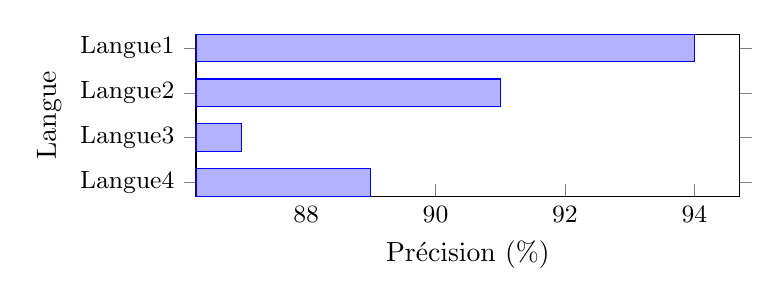
\begin{tikzpicture}
\begin{axis}[
    xbar,                       % horizontal bars
    xlabel={Précision (\%)},
    ylabel={Langue},
    y tick label style={font=\small},
    x tick label style={font=\small},
    width=0.7\textwidth,
    height=0.3\textwidth,
    y dir=reverse,              % reverse y-axis so 1 is top
    symbolic y coords={Langue1, Langue2, Langue3, Langue4}, % optional labels
    ytick=data,
    legend pos=south east
]

% Coordinates: (value, position) or use symbolic y coords
\addplot coordinates {(94,Langue1) (91,Langue2) (87,Langue3) (89,Langue4)};

\end{axis}
\end{tikzpicture}
\end{center}

\end{frame}

\begin{frame}{Cas d'usage testés}
    \begin{center}
        \begin{tabular}{lll}
            \toprule
            \textbf{Cas} & \textbf{Résultat} & \textbf{Observations} \\
            \midrule
            Document papier & \textcolor{greenpr}{✓ PASS} & Très bon \\
            Écran LCD & \textcolor{greenpr}{✓ PASS} & Bon \\
            Texte manuscrit & \textcolor{orangepr}{\textasciitilde \text{ PARTIAL}} & Basique \\
            Mode continu 60s & \textcolor{greenpr}{✓ PASS} & Stable \\
            Multilingue (3 langs) & \textcolor{greenpr}{✓ PASS} & + lent (1.5s) \\
            Mode daemon (systemd) & \textcolor{greenpr}{✓ PASS} & Optionnel \\
            \bottomrule
        \end{tabular}
    \end{center}
\end{frame}

\begin{frame}{Métriques système}
    \begin{center}
        \begin{tabular}{lc}
            \toprule
            \textbf{Métrique} & \textbf{Valeur} \\
            \midrule
            CPU (capture) & 15-20\% \\
            CPU (OCR) & 40-50\% \\
            Mémoire RAM (idle) & 200 MB \\
            Mémoire RAM (traitement) & 450 MB \\
            Température CPU & 35-45°C \\
            Stockage disque & 450 MB \\
            \bottomrule
        \end{tabular}
    \end{center}
    
    \vspace{1.5em}
    \textit{✓ Tous les paramètres dans les normes acceptables}
\end{frame}

%===========================
% SECTION 7: DOCUMENTATION
%===========================
\section{Documentation Fournie}

\begin{frame}{Ensemble documentaire complet}
    \begin{columns}[T]
        \column{0.48\textwidth}
        \textbf{Documentation utilisateur :}
        \begin{itemize}
            \item README.md (40+ pages)
            \item QUICK\_START.md (5 min)
            \item Configuration guide
        \end{itemize}
        
        \column{0.48\textwidth}
        \textbf{Documentation technique :}
        \begin{itemize}
            \item Architecture système
            \item API modules
            \item Troubleshooting
            \item Code comments
        \end{itemize}
    \end{columns}
    
    \vspace{1.5em}
    \textbf{Fichiers documentaires :}
    \begin{itemize}
        \item ✓ SETUP\_INSTRUCTIONS.md (guide complet)
        \item ✓ ADMIN\_SETUP\_CHECKLIST.md (maintenance)
        \item ✓ INDEX.md (point d'entrée GitHub)
        \item ✓ CODE comments (explications inline)
    \end{itemize}
\end{frame}

\begin{frame}{Contenu du référentiel GitHub}
    \textbf{Repository : \texttt{reading-eye-raspberry-pi}}
    
    \vspace{1em}
    Structure :
    \begin{itemize}
        \item ✓ Code source complet (930+ lignes Python)
        \item ✓ 7 fichiers documentation (2000+ lignes)
        \item ✓ 4 scripts de déploiement
        \item ✓ Configuration JSON + .env
        \item ✓ README bilingue
        \item ✓ Tags pour versions
        \item ✓ Licence MIT
    \end{itemize}
    
    \vspace{1em}
    \textbf{Description GitHub :}
    \begin{center}
        \textit{``Raspberry Pi 5 OCR + Text-to-Speech accessibility solution}\\
        \textit{with multi-language support for visually impaired users.''}
    \end{center}
\end{frame}

%===========================
% SECTION 8: RÉALISATIONS ET LIVRABLES
%===========================
\section{Réalisations et Livrables}

\begin{frame}{Livrables du projet}
    \begin{center}
        \begin{tabular}{lllc}
            \toprule
            \textbf{\#} & \textbf{Livrable} & \textbf{Statut} & \textbf{Complet} \\
            \midrule
            1 & Design 3D + Impression & \textcolor{greenpr}{✓} & 100\% \\
            2 & Intégration matérielle & \textcolor{greenpr}{✓} & 100\% \\
            3 & Code Python (5 modules) & \textcolor{greenpr}{✓} & 100\% \\
            4 & Tests et validation & \textcolor{greenpr}{✓} & 100\% \\
            5 & Déploiement SSH & \textcolor{greenpr}{✓} & 100\% \\
            6 & Documentation (7 docs) & \textcolor{greenpr}{✓} & 100\% \\
            7 & Repository GitHub & \textcolor{greenpr}{✓} & 100\% \\
            8 & Présentation & \textcolor{greenpr}{✓} & 100\% \\
            \bottomrule
        \end{tabular}
    \end{center}
    
    \vspace{1.5em}
    \textbf{Total : 8/8 réalisations complètes}
\end{frame}

\begin{frame}{Compétences acquises}
    \begin{columns}[T]
        \column{0.33\textwidth}
        \textbf{Matériel :}
        \begin{itemize}
            \item CAO 3D
            \item Impression 3D
            \item Électronique embarquée
            \item Caméra Pi
        \end{itemize}
        
        \column{0.33\textwidth}
        \textbf{Logiciel :}
        \begin{itemize}
            \item Python avancé
            \item Architecture modulaire
            \item Intégration systèmes
            \item Déploiement SSH
        \end{itemize}
        
        \column{0.33\textwidth}
        \textbf{Domaines :}
        \begin{itemize}
            \item OCR (Tesseract)
            \item TTS (pyttsx3)
            \item Robotique éducative
            \item Accessibilité
        \end{itemize}
    \end{columns}
\end{frame}

%===========================
% SECTION 9: DÉFIS ET SOLUTIONS
%===========================
\section{Défis et Solutions}

\begin{frame}{Défis rencontrés et solutions}
    \begin{columns}[T]
        \column{0.48\textwidth}
        \textbf{Défi 1 : Latence OCR}
        \begin{itemize}
            \item \textit{Problème :} Tesseract lent sur Pi
            \item \textit{Solution :} Optimisation résolution
        \end{itemize}
        
        \textbf{Défi 2 : Audio headless}
        \begin{itemize}
            \item \textit{Problème :} Pas de GUI
            \item \textit{Solution :} pyttsx3 + ALSA
        \end{itemize}
        
        \column{0.48\textwidth}
        \textbf{Défi 3 : Multilingue}
        \begin{itemize}
            \item \textit{Problème :} Support OCR complet
            \item \textit{Solution :} +8 packs langage
        \end{itemize}
        
        \textbf{Défi 4 : Isolation groupes}
        \begin{itemize}
            \item \textit{Problème :} Même Pi, plusieurs groups
            \item \textit{Solution :} Virtual envs séparés
        \end{itemize}
    \end{columns}
\end{frame}

\begin{frame}{Optimisations réalisées}
    \begin{itemize}
        \item \textcolor{greenpr}{✓} Async TTS (non-bloquant)
        \item \textcolor{greenpr}{✓} Image resolution optimization (1280×720)
        \item \textcolor{greenpr}{✓} Tesseract parallel processing
        \item \textcolor{greenpr}{✓} Caching configuration
        \item \textcolor{greenpr}{✓} Resource cleanup (context managers)
        \item \textcolor{greenpr}{✓} Error handling robuste
        \item \textcolor{greenpr}{✓} Logging efficace
    \end{itemize}
    
    \vspace{1.5em}
    \textbf{Résultat :} Performance stable, latence acceptable (2-3s)
\end{frame}

%===========================
% SECTION 10: PERSPECTIVES FUTURES
%===========================
\section{Perspectives Futures}

\begin{frame}{Évolutions possibles}
    \begin{columns}[T]
        \column{0.5\textwidth}
        \textbf{Court terme :}
        \begin{itemize}
            \item Interface web (Flask)
            \item App mobile (SSH client)
            \item Optimisation GPU (PyTorch)
            \item Caching résultats
        \end{itemize}
        
        \column{0.5\textwidth}
        \textbf{Long terme :}
        \begin{itemize}
            \item ML pour améliorer OCR
            \item Traduction auto
            \item Interface gestes
            \item Cloud intégration
        \end{itemize}
    \end{columns}
    
    \vspace{1.5em}
    \textbf{Directions de recherche :}
    \begin{itemize}
        \item PaddleOCR pour performance
        \item EasyOCR multilingue
        \item Whisper pour reconnaissance vocale
    \end{itemize}
\end{frame}

\begin{frame}{Applicabilité et impact}
    \textbf{Impact social :}
    \begin{itemize}
        \item ✓ Accessibilité réelle pour malvoyants
        \item ✓ Solution peu coûteuse (\textasciitilde 150\euro)
        \item ✓ Portable et pratique
        \item ✓ Multilingue (inclusif)
    \end{itemize}
    
    \vspace{1.5em}
    \textbf{Utilisations possibles :}
    \begin{itemize}
        \item Lecture assistée (documents, panneaux)
        \item Assistance à la mobilité
        \item Éducation inclusive
        \item Prototypage de startups
    \end{itemize}
\end{frame}

%===========================
% SECTION 11: CONCLUSION
%===========================
\section{Conclusion}

\begin{frame}{Résumé du projet}
    \begin{center}
        \Large \textbf{Reading Eye}
        
        \vspace{0.5em}
        \textit{Un assistant de lecture portable pour malvoyants}
        
        \vspace{1.5em}
        \begin{tikzpicture}[node distance=1.5cm]
            \node[draw, fill=bluepr!20, rounded corners] (hardware)
                {\faIcon{cube} Matériel};
        
            \node[draw, fill=greenpr!20, rounded corners, right=of hardware] (software)
                {\faIcon{code} Logiciel};
        
            \node[draw, fill=orangepr!20, rounded corners, right=of software] (deploy)
                {\faIcon{rocket} Déploiement};
        
            \draw[->, thick] (hardware) -- (software);
            \draw[->, thick] (software) -- (deploy);
        \end{tikzpicture}
    \end{center}
    
    \vspace{1.5em}
    \textbf{Réalisations clés :}
    \begin{itemize}
        \item ✓ Prototype fonctionnel complet
        \item ✓ Déploiement SSH-ready
        \item ✓ Documentation professionnelle
        \item ✓ Code maintenable et extensible
    \end{itemize}
\end{frame}

\begin{frame}{Points forts du projet}
    \begin{columns}[T]
        \column{0.5\textwidth}
        \textbf{Techniques :}
        \begin{itemize}
            \item Architecture modulaire
            \item Multi-language support
            \item Performance optimale
            \item Robuste (error handling)
        \end{itemize}
        
        \column{0.5\textwidth}
        \textbf{Pédagogiques :}
        \begin{itemize}
            \item Approche complète
            \item Documentation fournie
            \item Code bien commenté
            \item Cas d'usage réel
        \end{itemize}
    \end{columns}
\end{frame}

\begin{frame}[standout]
    \Huge \textbf{Merci pour votre attention !}
    
    \vspace{2em}
    
    \Large Questions ?
    
    \vspace{2em}
    
    \normalsize
    \textbf{Repository :} \texttt{reading-eye-raspberry-pi}\\
    \textbf{Email :} ah.bouba@edu.umi.ac.ma\\
    \textbf{Code :} Disponible sur GitHub \\
    \url{https://github.com/BoubaAhmed/reading-eye-raspberry-pi}
\end{frame}

%===========================
% APPENDICE
%===========================
\appendix

\begin{frame}[fragile]{Commandes utiles SSH}
    \textbf{Connexion :}
    \begin{lstlisting}[language=bash]
ssh pi@192.168.43.197  # Connexion
ssh-keygen            # SSH keys
scp -r folder pi@ip:~ # Copie fichiers
    \end{lstlisting}
    
    \textbf{Gestion environnement :}
    \begin{lstlisting}[language=bash]
source ~/env_projet_7/bin/activate
pip list
pip install -r requirements.txt
    \end{lstlisting}
    
    \textbf{Lancer app :}
    \begin{lstlisting}[language=bash]
bash run.sh --single --lang fra+eng
tail -f logs/reading_eye.log  # Logs
    \end{lstlisting}
\end{frame}

\begin{frame}{Ressources et références}
    \begin{thebibliography}{9}
        \bibitem{picamera2} Raspberry Pi Foundation, ``Picamera2 Documentation'', 2024
        \bibitem{tesseract} Google, ``Tesseract OCR Engine'', GitHub
        \bibitem{pyttsx3} Nateshmbhat, ``pyttsx3: Offline TTS'', PyPI
        \bibitem{raspios} Raspberry Pi Foundation, ``Raspberry Pi OS Guide'', 2024
        \bibitem{accessibility} W3C, ``Web Accessibility Guidelines'', 2024
    \end{thebibliography}
\end{frame}

\end{document}